\RequirePackage{luatex85}
\documentclass[tikz]{standalone}
% Default preamble
\usepackage{pgfplots}
\pgfplotsset{compat=newest}
\usepgfplotslibrary{groupplots}
\usepgfplotslibrary{polar}
\usepgfplotslibrary{smithchart}
\usepgfplotslibrary{statistics}
\usepgfplotslibrary{dateplot}
\usepgfplotslibrary{ternary}
\usepackage[T1]{fontenc}
\begin{document}
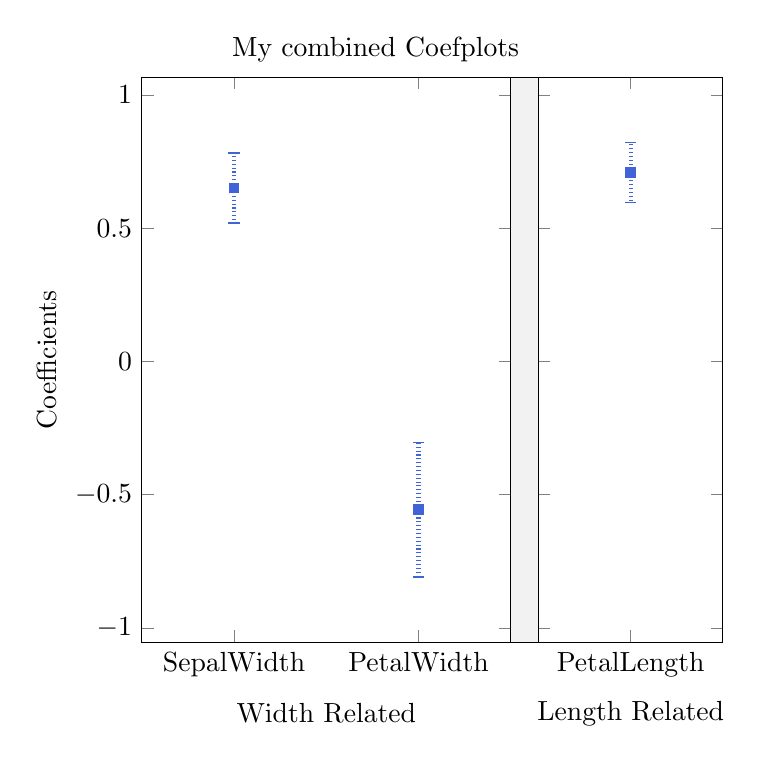
\begin{tikzpicture}
\begin{groupplot}[group style={group size={2 by 1}, y descriptions at={edge left}, ylabels at={edge left}, horizontal sep={10pt}}, ymin={-1.053030052084214}, ymax={1.0656974335865952}, ylabel={Coefficients}, ylabel style={}]
    \nextgroupplot[xticklabel style={}, yticklabel style={}, width={133.33333333333331pt}, height={204pt}, symbolic x coords={SepalWidth,PetalWidth}, xtick={SepalWidth,PetalWidth}, xmin={{[normalized]-0.5}}, xmax={{[normalized]1.5}}, scale only axis]
    \addplot[only marks, mark={square*}, mark options={mark size={1.75pt}, line width={0pt}, fill={rgb,255: red, 64; green, 99; blue, 216}, fill opacity={1}, draw={rgb,255: red, 64; green, 99; blue, 216}, draw opacity={1}}, error bars/error mark={|}, error bars/error mark options={mark size={2.0pt}, solid, line width={0.6pt}, fill={rgb,255: red, 64; green, 99; blue, 216}, fill opacity={1}, draw={rgb,255: red, 64; green, 99; blue, 216}, draw opacity={1}}, error bars/error bar style={draw={rgb,255: red, 64; green, 99; blue, 216}, draw opacity={1}, densely dotted, line width={1.5pt}}, draw={rgb,255: red, 64; green, 99; blue, 216}, draw opacity={1}, line width={0.5pt}, error bars/y dir={both}, error bars/y explicit]
        coordinates {
            (SepalWidth,0.6508371593133089) +- (0,0.1317182882857669)
            (PetalWidth,-0.5564826601669999) +- (0,0.25207883587827457)
        }
        ;
    \nextgroupplot[xticklabel style={}, yticklabel style={}, width={66.66666666666666pt}, height={204pt}, symbolic x coords={PetalLength}, xtick={PetalLength}, xmin={{[normalized]-0.5}}, xmax={{[normalized]0.5}}, scale only axis]
    \addplot[only marks, mark={square*}, mark options={mark size={1.75pt}, line width={0pt}, fill={rgb,255: red, 64; green, 99; blue, 216}, fill opacity={1}, draw={rgb,255: red, 64; green, 99; blue, 216}, draw opacity={1}}, error bars/error mark={|}, error bars/error mark options={mark size={2.0pt}, solid, line width={0.6pt}, fill={rgb,255: red, 64; green, 99; blue, 216}, fill opacity={1}, draw={rgb,255: red, 64; green, 99; blue, 216}, draw opacity={1}}, error bars/error bar style={draw={rgb,255: red, 64; green, 99; blue, 216}, draw opacity={1}, densely dotted, line width={1.5pt}}, draw={rgb,255: red, 64; green, 99; blue, 216}, draw opacity={1}, line width={0.5pt}, error bars/y dir={both}, error bars/y explicit]
        coordinates {
            (PetalLength,0.7091319591367299) +- (0,0.11209691841092581)
        }
        ;
\end{groupplot}
\coordinate (freeze) at (current bounding box.south);
\coordinate (title) at (current bounding box.north);
\filldraw[fill=gray, draw=black,fill opacity=0.1] (group c1r1.north east) rectangle (group c2r1.south west);
\node[yshift=-1em] at ({group c1r1.center}|-{freeze}) {Width Related};
\node[yshift=-1em] at ({group c2r1.center}|-{freeze}) {Length Related};
\node[yshift=1em] at (title) {My combined Coefplots};
\end{tikzpicture}
\end{document}
